%
% auth: Mattijs Korpershoek
% mail: <mattijs.korpershoek@gmail.com>
%

\section{Context}

\subsection{Company}
\begin{frame}
    \frametitle{Company}
    \begin{minipage}{0.49\textwidth}
        \begin{itemize}
            \item Hired by Celad
            \item Intel is one of Celad's client
            \item Android for Intel platforms
        \end{itemize}
    \end{minipage}
    \begin{minipage}{0.49\textwidth}
        \flushright
        
\includegraphics[height=1cm]{../../report/src/img/logocelad.jpg} \\[0.5cm]
        
\includegraphics[height=1cm]{../../report/src/img/logointel.jpg} \\[0.5cm]
        
\includegraphics[height=1cm]{./img/androidLogo.png}
    \end{minipage}
\end{frame}

\subsection{Hal \& Android}
\begin{frame}
    \frametitle{Android architecture}
    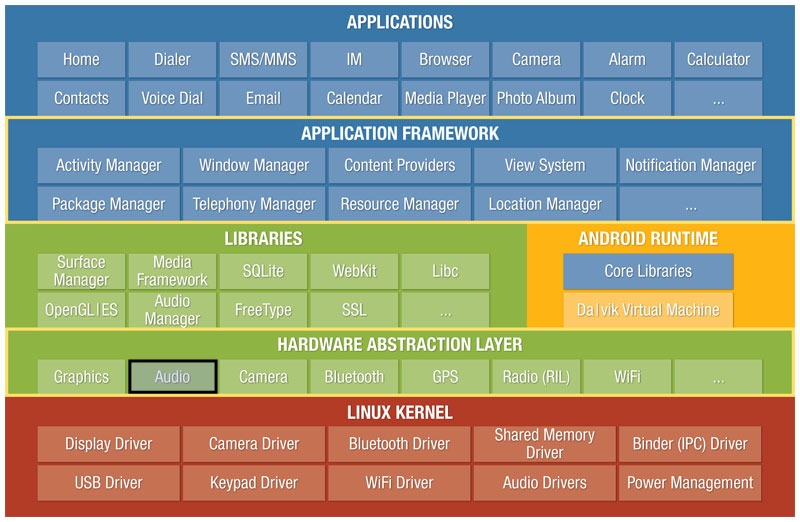
\includegraphics[width=\textwidth]{../../report/src/img/android-archi-audio-hal.jpeg}
\end{frame}

\begin{frame}
    \frametitle{Intel Audio HAL}
    \begin{minipage}{0.40\textwidth}
        \begin{block}{Hardware Abstraction Layer}
            \begin{itemize}
                \item Userland solution
                \item Fully configurable without code modification
            \end{itemize}
        \end{block}
    \end{minipage}
    \begin{minipage}{0.50\textwidth}
        \flushright
        % report must be compiled before this works
        % TODO uncomment this
        \includegraphics[height=0.85\textheight]{../../report/src/img/hal-architecture.pdf}
    \end{minipage}
\end{frame}


\subsection{Parameter-framework}
\begin{frame}
    \frametitle{Parameter-framework structure}
    \begin{minipage}{0.40\textwidth}
    \begin{block}{Structure description}
        \begin{itemize}
            \item Structured in a tree
            \item XML description
            \item Parameter definitions
        \end{itemize}
    \end{block}
    \end{minipage}
    \begin{minipage}{0.50\textwidth}
            \dirtree{%
                .1 audio.
                    .2 microphone.
                        .3 echo\_cancellation.
                            .4 enable.
                            .4 configuration.
                                .5 gain.
                                .5 coefficient.
                    .2 speaker.
                        .3 equalizer.
                            .4 enable.
                            .4 configuration.
                                .5 filter.
                                .5 coefficient.
            }
    \end{minipage}
\end{frame}

\begin{frame}
    \frametitle{Parameter-framework settings}
    \begin{minipage}{0.40\textwidth}
    \begin{block}{Domains description}
        \begin{itemize}
            \item Settings description
            \item Based on criteria
        \end{itemize}
    \end{block}
    \end{minipage}
    \begin{minipage}{0.53\textwidth}
        % [WORKAROUND] use of inputlisting since normal listing are not compiling
        \lstinputlisting[language=pfwLang]{./code/example.pfw}
    \end{minipage}
\end{frame}
